\section{Script SQL (DDL) de création de la base de données}
\subsection{Création des tables: explications}
Le code infra permet de créer les tables et leurs attributs respectifs. Pour chaque table, les clefs primaires et étrangères ont été établies. Certaines contraintes ont été rejetées par PhpMyAdmin, mais pourront être gérées via le code php.

\subsection{Code de création des tables}
\inputminted[breaklines =true, autogobble, linenos, frame = single]{sql}{Codes/code_creation.tex}

\subsection{Code de création des clés étrangères}
\inputminted[breaklines =true, autogobble, linenos, frame = single]{sql}{Codes/code_key.tex}

Le résultat de ce script dans phpMyAdmin:voir figure \ref{fig:pmy_creation_fk}.

\subsection{Diagramme de relation entre les entités}
\begin{figure}[H]
    \centering
    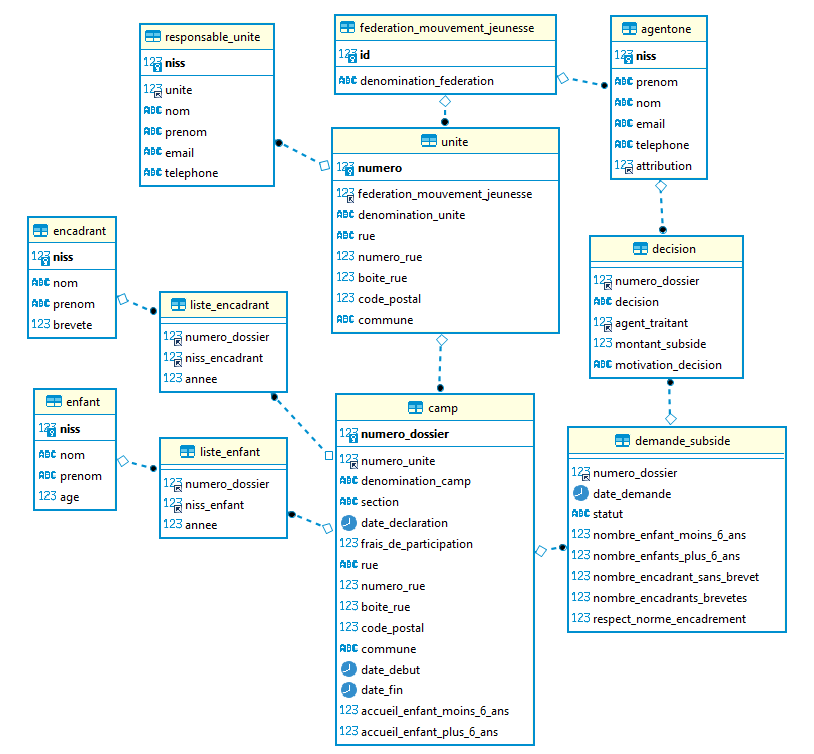
\includegraphics[width=17cm]{Pictures/er_diagram.png}
    \caption{Vue Dbeaver sur la base de données globale, avec relation entre les entités.}
    \label{fig:er_diagram}
\end{figure}



\section{Élément de SQL avancés}
\subsection{Prédicats: check des tables}
\subsubsection{Vérifications sur les dates de camps}
Un premier check permet de vérifier que la date de fin est bien cohérente avec la date de début.

%ajouter code 

Un deuxième permet de ne pas introduire de demande de subsides tant que le camp ne s'est pas terminé. 

%ajouter code


Concernant les dates calendrier (30 avril, 30 septembre) où la déclarations ou la demande de subsides doit être rentrées, elle se gérera au niveau du formulaire. 

Nous n'avons pas implémenté non plus le check sur les conflits de dates concernant les présences; une possibilité est d'ajouter des attributs de date dans la table liste\_enfant et liste\_encadrant.

\subsubsection{vérifications sur les âges}
Concernant les enfants et les encadrants, la première liste ne doit présenter que des enfants de moins de 15 ans, tandis que la seconde d'au moins 16 ans.



\subsection{Les vues}

\subsubsection{Vue pour les fédérations sur les unités fédérés}




\subsubsection{Vue uniquement sur les camps d'une unité précise}



\subsubsection{Vue sur les dossiers d'un agent (en fonction de sa fédération)}








\subsection{Les triggers}
\subsubsection{Attribution d'un dossier à un agent ONE}

\subsubsection{Calcul du nombre de participant lorsqu'une demande de subsides a été rentrée}




\subsection{droit d'accès}
\subsubsection{Agent ONE}
Accès à toutes les tables
\inputminted[breaklines =true, autogobble, linenos, frame = single]{sql}{Codes/code_role_agent_one.tex}



\subsubsection{Responsable d'unité}
Accès uniquement à son unités: en modification camps déclarés, demandes de subsides. En consultation: décision de l'ONE. 



\subsubsection{Animateurs d'unité}
Accès uniquement en consultation à son unités et à ses camps. 






%\subsection{Contraintes de clefs primaires, uniques, externes}




\section{Script SQL (insert)}